\documentclass[10pt,a4paper,english]{article}

\usepackage[utf8]{inputenc}
\usepackage{amsmath}
\usepackage{graphicx}
\usepackage{geometry}
\usepackage{hyperref}
\usepackage{cite}
\usepackage{ragged2e}
\usepackage{xcolor}
\usepackage{listings}
\usepackage{comment}
\usepackage{wrapfig}

\graphicspath{{images/}}

\lstset{
    numbers=none,
    tabsize=3,
    breaklines=true,
    basicstyle=\ttfamily,
    framerule=0pt,
    backgroundcolor=\color{gray!25},
    columns=fullflexible,
}

\hypersetup{
    colorlinks=true,
    linkcolor=blue,
    filecolor=magenta,      
    urlcolor=blue,
    pdftitle={ROS2_Investigation},
    }

\title{ROS2 Investigation}
\author{Alexander Armstrong}
\date{\today}

\begin{document}

% Title Page
\begin{titlepage}
    \centering
    \vspace*{2cm}
    
    {\Huge\bfseries ROS2 Investigation\par}
    \vspace{1.5cm}
    
    {\Large Technical Analysis and Implementation Study\par}
    \vspace{2cm}
    
    {\large\itshape Alexander Armstrong\par}
    \vspace{1cm}
    
    {\large Russel Mineral Equipment\par}
    \vspace{0.5cm}
    
    {\large Email: Alex.Armstrong@rmeglobal.com\par}
    \vspace{2cm}
    
    \vfill
    
    {\large \today\par}
    
    \vspace{1cm}
    
\end{titlepage}

% Optional: Add table of contents
\tableofcontents
\newpage

\section{Executive Summary}

This investigation presents a comprehensive analysis of Robot Operating System 2 (ROS2) implementation for industrial mill relining simulation, specifically through the development and deployment of a kinematic model similar to the RME Russel 7. The research addresses the potential for ROS2 integration into RME's current software usage for kinematic model visualisation, calculations and Mill Reliner path planning. The primary contribution of this body of work lies in the successful integration of ROS2's distributed computing architecture with the MoveIt2 motion planning framework to create a robust testing ground for Mill Reliner operations. The implemented system demonstrates basic kinematic modeling and inverse kinematic calculations, with potential for collision avoidance capabilities in future development. The open-source nature of ROS2, MoveIt2, and RViz2 leaves room for considerable improvement whilst creating cause for many compilation errors to arise from non-expert users. The modular nature of ROS2's use of URDF and Xacro files does enable large scalability across multiple mill configurations and has integration with current SolidWorks RME practices but ultimately designing a URDF file that accurately represents a mill relining machine is a complex task if done by hand. This investigation concludes that ROS2 provides a promising framework for enhancing the automation and efficiency of mill relining operations, but also highlights the challenges and complexities involved in its implementation.


\section{Introduction}
ROS is an operating system that was developed in 2007 and maintained until 2015 when it underwent a major revision of the ROS API to include new features and libraries like real-time computing and embedded system hardware integration henceforth known as ROS2. ROS2 has ports for Windows operation but was developed on Linux systems specifically designed for Ubuntu LTS versions. ROS2 aims to release a new version every year in May with only marginally small changes to that year's upgraded packages so as to not impact previous users implementation too significantly. \par

The advent of advanced robotic systems, coupled with sophisticated software frameworks such as Robot Operating System 2 (ROS2), presents opportunities for addressing critical operational challenges. ROS2, as a next-generation middleware platform, offers extensive capabilities in distributed computing and modular system architectures that are particularly well-suited for complex industrial automation applications. \par

This investigation presents a technical analysis of ROS2 implementation for autonomous mill relining operations through the development of a Russel 7-like manipulator system. It aims to construct the model and test its performance and accuracy in simulation environments. The main interest is the inverse kinematic calculations and joint representations associated. The research addresses fundamental questions regarding the feasibility, scalability, and viability of deploying advanced robotic models in the ROS environment. \par

\subsection{Problem Statement and Research Objectives}

The primary research objective centers on evaluating ROS2's capabilities and suitability across a number of key technical areas including:

\begin{enumerate}
    \item \textbf{Kinematic Complexity}: Development of accurate mathematical models for a hybrid kinematic chain incorporating both prismatic and revolute joints to achieve optimal workspace coverage within spatial constraints imposed by mill geometry.

    \item \textbf{Inverse Kinematic Calculations}: Implementation of robust inverse kinematic algorithms to compute joint configurations from end-effector positions, ensuring precise control over the manipulator's movements in 3 dimensional space.

    \item \textbf{Motion Planning Optimization}: Implementation of path planning algorithms within the defined joint and workspace constraints with potential for collision avoidance and sensor-based control systems.
    
    \item \textbf{System Integration}: Seamless integration of multiple software components including motion planning frameworks and kinematic calculations (MoveIt), hardware abstraction layers (ROS2 Control), and visualization tools (RViz2) within a unified system architecture.
\end{enumerate}

\subsection{Technical Approach and Methodology}

The implemented solution leverages ROS2's distributed node architecture to create a modular, scalable system comprising several key components:

\textbf{Kinematic Modeling}: The robotic system utilizes a 7-DOF configuration modelled to represent an appropriate approximation of the physical characteristics of a Russel 7. The kinematic chain consists of:
\begin{itemize}
    \item Prismatic beam joint enabling horizontal positioning across the mill width
    \item Revolute turntable providing 360° rotational coverage inside the mill
    \item Revolute pitch mechanism for vertical positioning of the boom
    \item Prismatic boom extension for horizontal reach adjustment
    \item Revolute slewing joint of the grapple assembly
    \item Revolute roll joint for orientation adjustment of the grapple
    \item Revolute pitch joint for tilting the grapple end effector pins
\end{itemize}

\textbf{Joint limits}: The kinematic model incorporates joint limits to ensure realistic movement constraints, preventing unrealistic configurations and ensuring safe operation within the mill environment. This includes defining maximum and minimum angles for revolute joints and limits for prismatic joints to avoid collisions and maintain operational safety as well as to prevent hardware damage from collisions.

\textbf{Inverse Kinematic Calculations}: The system implements inverse kinematic algorithms to compute joint angles from end-effector positions, ensuring precise control over the manipulator's movements in 3D space. The kinematic model is designed to handle both prismatic and revolute joints, allowing for flexible positioning and orientation of the end effector backwards to the base-link.

\textbf{Motion Planning Framework}: Integration with MoveIt2 provides access to motion planning algorithms including RRT-Connect (Rapidly-exploring Random Tree Connect) for efficient path generation in 3-Dimensional space. The system employs OMPL (Open Motion Planning Library) algorithms to optimise the trajectory planning process with potential future enhancements for collision avoidance. This integrations allows for users to set scenes and pre-defined motion plans, facilitating more complex task execution.

\textbf{Visualization and Simulation}: RViz2 integration provides comprehensive 3D visualization capabilities essential for system validation, operator training, and monitoring of robotic operations. RViz2 is the primary tool developed for ROS2 implementation and allows dynamic control over the node visualisation, enabling real-time feedback and debugging of the kinematic model and motion planning algorithms and inverse kinematics.

\newpage



\section{ROS2 Overview}

ROS2 is comprised of several key components, including:

\begin{enumerate}
    \item \textbf{Client Libraries}: Language-specific libraries (C++ and Python) that provide APIs for interacting with ROS2 features.
    \item \textbf{Nodes and Discovery}: Independent processes that communicate with each other using topics, services, and actions.
    \begin{itemize}
        \item \textbf{Topics}: Named channels for asynchronous message passing between nodes.
        \item \textbf{Services}: Synchronous request-response communication mechanism for inter-node interactions.
        \item \textbf{Actions}: Long-running tasks that can be preempted or cancelled, providing feedback during execution.
    \end{itemize}
    \item \textbf{Parameters}: Configuration settings that can be dynamically adjusted at runtime.
    \item \textbf{The Build System}: ROS2 uses CMake or Python setuptools as its build system, which is used to compile and link the source code of ROS2 packages.
    \item \textbf{Launch Files}: C++ or Python scripts that define how nodes are launched and configured, allowing for complex system setups.
    \item \textbf{URDF/Xacro}: Unified Robot Description Format (URDF) and Xacro files define the robot's physical structure, including joints, links, and their properties.
    \item \textbf{RViz2}: A visualization tool that allows users to visualize the robot's state, sensor data, and planned trajectories in a 3D environment.
    \item \textbf{MoveIt2}: A motion planning framework that integrates with ROS2 to provide advanced capabilities for robot motion planning, including trajectory generation, collision avoidance, and kinematic calculations.
\end{enumerate}

The full construction of the above system is visualised in Figure \ref{fig:nodes_topics_services}.
\begin{figure}[ht]
    \centering
    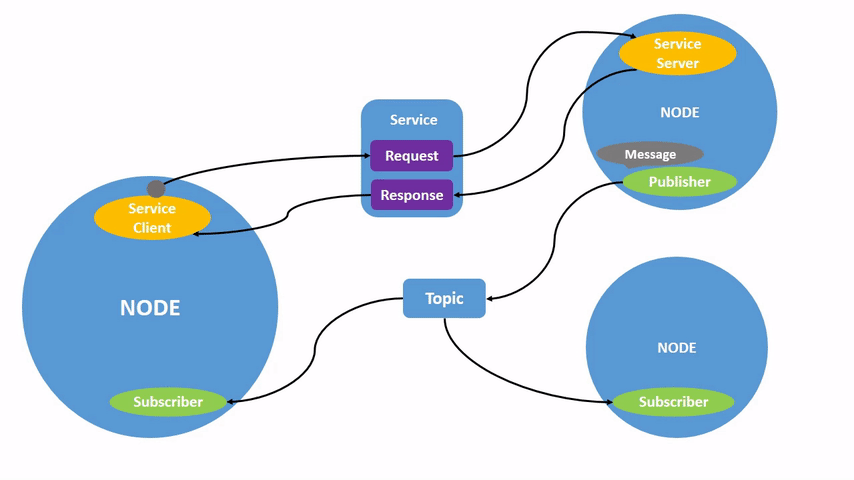
\includegraphics[width=1.0\textwidth]{Nodes_Topics_Services.png}
    \caption{Nodes and Topics/Services in ROS2}
    \label{fig:nodes_topics_services}
\end{figure}

\subsection{Client Libraries}
Client libraries in ROS2 provide the necessary APIs for developers to interact with the ROS2 framework using various programming languages. The most commonly used languages are C++ and Python, both are widely supported and have extensive documentation and community support. Python was exclusively used for this investigation's implementation due to its ease of use and rapid development capabilities as well as personal proficiency.
The common core ROS Client Library, the \texttt{rcl} library, is an interface that provides logic and behavior of ROS concepts that is not language specific. As a result, further libraries only need to wrap the common RCL functionalities into their language specific function interfaces. The \texttt{rclcpp} library is the C++ client library, while the \texttt{rclpy} library serves as the Python client library. It is not required to use both libraries in the same project, but it is possible to use both C++ and Python nodes in the same ROS2 system. This allows for flexibility in choosing the most suitable language for each component of the system, depending on the specific requirements and constraints of the application.

\subsection{Nodes and Discovery}
A node is a fundamental building block of a ROS2 system, representing an independent process that can communicate with other nodes. Each node can publish data to deliver to other nodes or subscribe to named \textit{topics} to receive data from other nodes. For small/quick processes nodes can act as \textit{service} client to request other nodes to perform computations on their behalf or \textit{service} servers to perform the aforementioned functionality. For longer/more complex running processes nodes can also execute \textit{actions} which are able to provide feedback during operation. Nodes are designed to be modular and reusable, allowing developers to create complex systems by combining multiple nodes. In this investigation, nodes were used to implement the kinematic model, motion planning algorithms, and visualization components. \par
Discovery in ROS2 refers to the mechanisms that allow nodes to find and communicate with each other. This is essential for establishing the dynamic connections between nodes in a distributed system. When a new node is started it annouces its presence to other nodes on the same ROS Domain ID (a unique identifier for a ROS2 network) and recieves information from the other currently operating nodes so thatthe appropriate connections can be established. Nodes also periodically refresh their discovery information to ensure that the system remains up to date with the current state of the network. Nodes will also inform the network when they are going offline.

\subsection{Topics}
Topics are used for continuous data streams between nodes. Topics do not have to maintain a 1-1 relationship between publishers and subscribers, allowing for multiple nodes to publish to the same topic or subscribe to the same topic. This is useful for scenarios where multiple sensors are providing data that needs to be processed by a single node or where a single sensor's data needs to be consumed by multiple nodes. Topics are defined by a unique name and a message type, which specifies the structure of the data being transmitted. These messages are anonymous and do not require the sender and receiver to know about each other, allowing for loose coupling between nodes. This decoupling enables greater flexibility and scalability in the system architecture, as nodes can be added, removed or even replaced silently without affecting the overall functionality of the system.

\subsection{Services}
    \begin{itemize}
    \item \textbf{Service Servers} \par
    A service server is a node that provides a specific functionality or computation that can be requested by other nodes. It listens for incoming service requests and processes them, returning a response to the requesting node. Service servers are typically used for tasks that require a request-response interaction, such as querying the state of a robot or performing a specific computation. 
    \item \textbf{Service Clients} \par
    A service client is a node that sends a request to a service server and waits for a response, hence why services should only be small tasks, as processes are usually suspended whilst waiting for a response. It initiates the interaction by calling the service and receiving the result. Service clients are used to access the functionality provided by service servers, allowing nodes to perform computations or retrieve information from other nodes in the system.
    \end{itemize}

\subsection{Actions}
    \begin{itemize}
    \item \textbf{Action Server} \par
    An action server is a node that provides a long-running task that can be preempted or cancelled. It performs usually long and complex task whilst providing feedback during the execution of the action. Action servers are useful for tasks that require continuous monitoring or feedback, such as motion planning or trajectory execution. They provide a way to manage complex operations that may take a significant amount of time to complete.
    \item \textbf{Action Client} \par
    An action client is a node that sends a goal to an action server and waits for a result. It initiates the interaction by calling the action and receiving feedback during the execution. Action clients are used to access the functionality provided by action servers, allowing nodes to perform complex tasks that require ongoing communication and coordination.
    \end{itemize}

\subsection{Parameters}
Parameters are configuration settings that are associated with nodes and set during startup but can be modified during runtime. Parameters allow for dynamic adjustment of node behaviour without direct changes to the code. Parameters are addressed by \texttt{node name}, \texttt{node namespace}, \texttt{parameter name}, and (optionally) \texttt{parameter namespace}. \par
A node must declare all of its parameters that it will accept during its lifetime. This declaration ensures that the node is less likely to encounter errors during runtime due to misconfigurations. Certain nodes may need to be configured without knowing all of their parameters at the time of declaration and in this case can be instantiated with a special declaration but this is not recommended as it can lead to unexpected behaviour for non expert users. \par

\subsection{The Build System}
The ROS2 build system is comprised of three components: the Build tool, the Build helper, and the Meta-Build tool. ROS2 relies heavily on dividing code into several \texttt{packages}, with each package containing a manifest file (package.xml). The manifest file contains the metadata about the package, including its dependencies on other packages. This manifest is required for the Meta-Build tool to function.

\begin{itemize}
    \item \textbf{Build Tool}
    The build tool is software the controls the compilation and testing of a single package. ROS2 will usually use CMake for C++ packages and setuptools for Python packages.
    \item \textbf{Build Helper}
    The build helper is a set of functions that hook into the build tool to aid the developers. The most common, also the package used in this investigation, is the \texttt{ament\_package}, which provides a set of macros and functions to simplify the build process. It helps with tasks such as finding dependencies, generating configuration files, and managing build options. The ament package will somewhat vary depending on the language used for the package, but the core functionality remains the same. A CMake package will use the \texttt{ament\_cmake} package and accompanying CMake description file, while a Python package will use the \texttt{setuptools} package.
    \item \textbf{Meta-Build Tool}
    This is a piece of software that knows how to topologically order a group of packages, and build or test them in the correct dependency order. This software will call into the Build Tool to do the actual work of compiling, testing, and installing the package. In ROS 2, the tool named colcon is used for this.
\end{itemize}

\subsection{Launch Files}
ROS2 systems are typically composed of many nodes that need to be launched and configured to form a complete system. This could technically be done by manually starting each node in he correct order and with its corresponding correct parameters but this is extremely impractical for larger systems. Launch files are used in this instance to perform the above in an automated and most importantly repeatable manner. They can be written in XML or Python and specify the nodes to be launched, their parameters, and any dependencies between nodes. They can also include conditional logic to control the execution of nodes based on specific conditions, making them flexible and adaptable to different scenarios. In this investigation, launch files were used to define the kinematic model, motion planning algorithms, and visualization components, allowing for a modular and scalable system architecture.

\subsection{URDF/Xacro}
URDF (Unified Robot Description Format) and Xacro (XML Macros) are used to describe the robot's physical structure, including its joints, links, and other properties. URDF files are XML-based representations that define the kinematic and dynamic properties of the robot, while Xacro files allow for more complex configurations and reusability of components through the use of macros. Xacro is particularly ideal for large and complex robot models, as the URDF files will become unwieldy and difficult to manage.

\subsection{RViz2}
RViz2 is a visualization tool that allows users to visualize the robot's state, sensor data, and planned trajectories in a 3D environment. It provides a graphical interface for monitoring the robot's state and debugging motion planning algorithms. RViz2 supports various visualization types, including 3D models, point clouds, and trajectories, making it a versatile tool for developing and testing robotic applications. In this investigation, RViz2 was used to visualize the kinematic model and motion planning, providing a comprehensive view of the system's state and performance.

\subsection{MoveIt2}
MoveIt2 is a motion planning framework that integrates with ROS2 to provide advanced capabilities for robot motion planning, including trajectory generation, collision avoidance, and kinematic analysis. It provides a set of tools and libraries for motion planning, manipulation, and perception, making it a powerful tool for developing robotic applications. MoveIt2 supports various motion planning algorithms, including RRT-Connect (Rapidly-exploring Random Tree Connect), which is used for efficient path generation in 3D space. It also provides interfaces for integrating with sensors, such as cameras and lidars, to enable perception capabilities in robotic systems. In this investigation, MoveIt2 was used to implement the motion planning algorithms for the kinematic model, allowing for real-time trajectory generation and optimization.

\newpage



\section{Environment Preparation}

\subsection{Ubuntu 24.04.2 LTS}
ROS2 is preferred to be run on Linux based systems and is primarily developed and tested on Ubuntu LTS (Long Term Support) versions. The latest version of ROS2, Kilted Kaiju, is compatible with Ubuntu 24.04.2 LTS, which provides a stable and reliable environment for ROS2 development. Ubuntu LTS versions are supported for five years, ensuring long-term stability and security updates. This investigation was conducted on Ubuntu 24.04.2 LTS to ensure compatibility with the latest ROS2 features and libraries.

\subsection{ROS2 Installation}
The installation of ROS2 on Ubuntu 24.04.2 LTS has extremely comprehensive \href{https://docs.ros.org/en/kilted/Installation.html}{documentation} available on the ROS2 website. The installation process can be done from binary packages, which are pre-compiled and ready to use, these are the recommended method for most users as it is ready to use, updates with systems and requires no compilation from the user post installation. Alternatively, ROS2 can be installed from source, which does allow for more customisation and control over the installation process but does require more technical knowledge and experience. The binary-desktop installation was used in this investigation to ensure a quick and easy setup process. It includes the core ROS2 packages, client libraries, and essential tools such as RViz2, some demos to assit the user in understanding ROS and codebases to build upon.

Installation from binary packages should result in a clean installation but there are a number of events that could result in a broken installation. If the installation is not working as expected, the documentation has a number of troubleshooting steps found at \href{https://docs.ros.org/en/kilted/Troubleshooting.html}{ROS2 Troubleshooting}.

Before any ROS2 program can be run the environment must be sourced. Every new terminal opened must source the environment and as such, for convenience it should be added to the user's bashrc file to ensure it is sourced automatically on every terminal startup. This can be done by entering the following command into any terminal: \begin{lstlisting}
  echo "source /opt/ros/kilted/setup.bash" >> ~/.bashrc 
\end{lstlisting} \par

\subsection{Creating a ROS2 Workspace and Package}
To create a ROS2 workspace, follow these steps:

1. Create a directory for the workspace:
\begin{lstlisting}
mkdir -p ~/ros2_ws/src
\end{lstlisting}

2. Navigate to the workspace directory:
\begin{lstlisting}
cd ~/ros2_ws
\end{lstlisting}

3. Create a package using the ROS2 package creation tool, noting this package will be built using python:
\begin{lstlisting}
ros2 pkg create --build-type ament_python --license Apache-2.0 my_package
\end{lstlisting}

This will create a new, mostly empty, package named \texttt{my\_package} in the \texttt{src} directory of the workspace as seen in Figure \ref{fig:my_package_folder}.
\begin{figure}[ht]
    \centering
    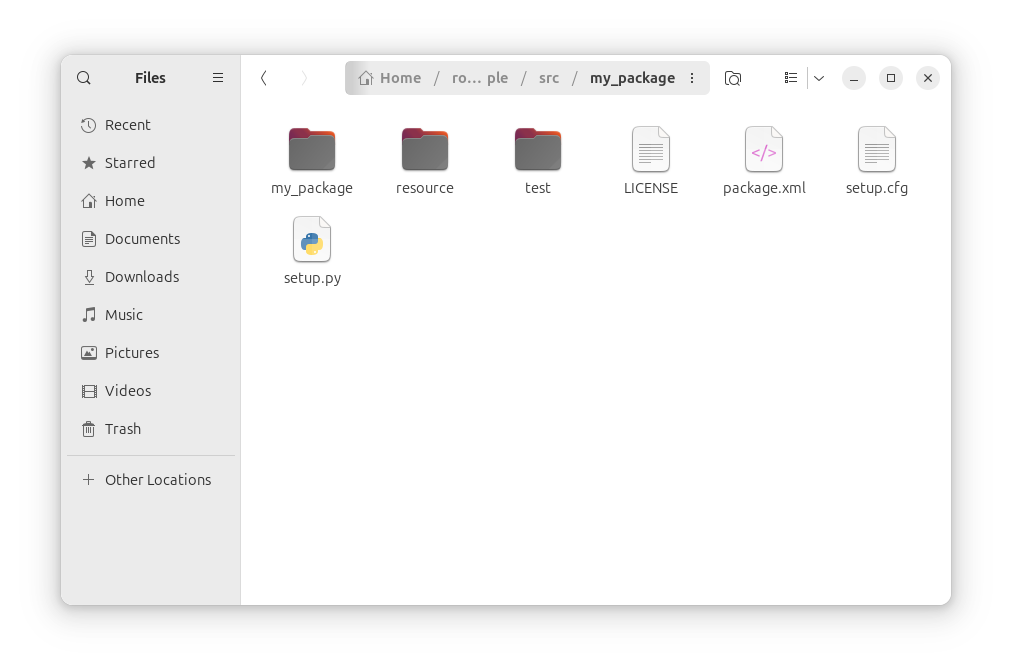
\includegraphics[width=1.0\textwidth]{my_package_folder.png}
    \caption{My Package Folder Structure}
    \label{fig:my_package_folder}
\end{figure}



\subsection{Colcon Build Tool}
The best way to build ROS2 packages is to use the \href{https://docs.ros.org/en/kilted/Tutorials/Beginner-Client-Libraries/Colcon-Tutorial.html}{colcon} build tool. It requires setting up a workspace, which is a directory that contains all the ROS2 packages to be built. The workspace must have a specific structure, with a \texttt{src} directory containing the source code of the packages. The colcon build tool will automatically detect the packages in the \texttt{src} directory and build them in the correct order based on their dependencies. The \texttt{src} directory can contain multiple packages and will change depending on the project's language. After the colcon build tool is run it will produce a set of new folders with build, install and log directories. The build directory contains the compiled code, the install directory contains the installed packages, and the log directory contains the build logs. The colcon build tool will also generate a \texttt{setup.bash} file in the install directory, which must be sourced to use the built packages in the workspace the same way the ROS2 environment is set up. This will need to be sourced after every build and as such should not be added to the bashrc file. The command to source the setup file is:
\begin{lstlisting}
source ~/ros2_ws/install/setup.bash
\end{lstlisting}
An example of the python workspace structure is shown in Figure \ref{fig:colcon_workspace_structure}.
\begin{figure}[ht]
    \centering
    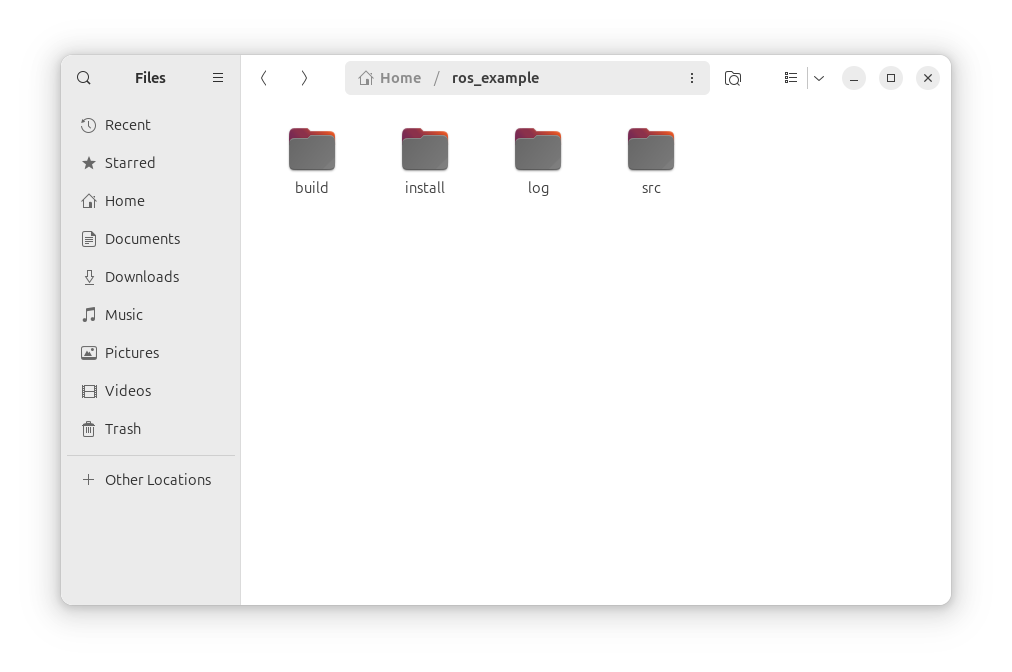
\includegraphics[width=1.0\textwidth]{colcon_build_folder.png}
    \caption{Colcon Workspace Structure}
    \label{fig:colcon_workspace_structure}
\end{figure} \par

\subsection{Launch file configuration}
In your new package, create a \texttt{launch} directory to store your launch files. This directory should contain a Python script that defines the nodes to be launched and their parameters. The launch file can be named anything but should have a \texttt{.py} extension. It is not necessary to have a single launch file for the entire package, multiple launch files can be created to seperate different functionalities which can then be included into a single master launch file if desired. This approach was used in this investigation to seperate the robot description (kinematic model), the moveit group configuration, the move group configuration and the controllers used in trajectory and path planning.

Launch files are explained in the \href{https://docs.ros.org/en/kilted/Tutorials/Intermediate/Launch/Creating-Launch-Files.html}{ROS2 Launch Documentation}. They have a number of standard includes such as \texttt{os} and \texttt{launch} followed by a function to define the launch, it will include the package directories, if multiple packages are being used, other files to be included at launch, and the node configurations themselves. 

After building with colcon, the launch file is then launched using the ROS command:
\begin{lstlisting}
ros2 launch my_package my_launch_file.py
\end{lstlisting}
Where \texttt{my\_package} is the name of the package containing the launch file and \texttt{my\_launch\_file.py} is the name of the launch file to be executed. This will start all the nodes defined in the launch file and configure them according to the specified parameters.

\newpage



\section{System Architecture}
\subsection{Kinematic Configuration - URDF Model}
The mill relining robot's kinematic configuration is represented using a Unified Robot Description Format (URDF) model, which defines the robot's physical structure, joint types, and link properties using XML syntax. The URDF model captures the essential characteristics of a Russel 7, including joint limits, inertial properties, and visual representations. This model was constructed by hand from a visual analysis and measurements of the RME Machine 592 from solidworks. URDF files can be generated from SolidWorks using the SW2URDF plugin, which automates the conversion of CAD models into URDF format, but this was not used in this investigation to protect RME's intellectual property.

Below is an example of the URDF configuration for the prismatic beam joint and horizontal beam link:
\begin{verbatim}
  <joint name="beam_joint" type="prismatic">
    <parent link="base_link"/>
    <child link="horizontal_beam"/>
    <origin xyz="0 0 1.5" rpy="0 0 0"/>
    <axis xyz="1 0 0"/>
    <limit lower="0" upper="5.5" effort="200" velocity="0.5"/>
  </joint>

  <link name="horizontal_beam">
    <visual>
      <origin xyz="1.3 0 0" rpy="0 0 0"/>
      <geometry>
        <box size="12.5 1.0 0.6"/>
      </geometry>
      <color rgba="1 0 1 1"/>
    </visual>
    <collision>
      <origin xyz="1.3 0 0" rpy="0 0 0"/>
      <geometry>
        <box size="12.5 1.0 0.6"/>
      </geometry>
    </collision>
    <inertial>
      <origin xyz="1.3 0 0" rpy="0 0 0"/>
      <mass value="15"/>
      <inertia ixx="0.011088" ixy="5E-06" ixz="0" iyy="0.001072" iyz="-0.000691" izz="0.011255" />
    </inertial>
  </link>
\end{verbatim}
The first field is the joint definition, its given a name and a type, prismatic in this case, allowing linear motion along an axis. Each joint has a relationship to the link before and after it, named the parent link and child link respectively. In this case, the parent link is the "base\_link" and the child link is the "horizontal\_beam". The origin specifies the position and orientation of the joint relative to its parent link, while the axis defines the direction of movement. The limit element sets constraints on the joint's range of motion.

The second field is the link definition, which describes the physical properties of the horizontal beam. It includes visual and collision geometry, inertial properties, and material specifications. The visual element defines how the link appears in simulation, while the collision element specifies its shape for collision detection purposes. The inertial element provides mass and inertia for dynamic simulation, enabling physics calculations during motion planning and execution.

This basic URDF configuration serves as the foundation for the kinematic model but can be vastly improved with the addition of XML formatted Macros, called Xacros. Xacros allow for more complex configurations and reusability of components, enabling the creation of modular and scalable robot models. The use of Xacros can significantly reduce redundancy in URDF files, making them easier to maintain and extend whilst increasing readability in most cases.

Consider the Inertia element in the URDF example above. The inertia matrix is defined as a 3x3 matrix representing the rotational inertia of the link about its principal axes. The values in the matrix are derived from the physical properties of the link, such as its mass distribution and geometry. In this case, the inertia matrix is explicitly defined with values for the diagonal elements (ixx, iyy, izz) and the off-diagonal elements (ixy, ixz, iyz) set to zero but this can be simplified using Xacro macros to define common inertial properties across multiple links. For example, a macro can be created to define the inertia matrix for all prismatic joints, allowing for consistent and efficient definition of inertial properties across the entire kinematic model. An example of such is depicted below:

\begin{verbatim}
  <xacro:macro name="box_inertia" params="m x y z">
    <inertia ixx="${m*(y*y+z*z)/12}" ixy="0" ixz="0"
             iyy="${m*(x*x+z*z)/12}" iyz="0"
             izz="${m*(x*x+y*y)/12}" />
  </xacro:macro>
\end{verbatim}

It can then replace the previous inertia definition, which was:
\begin{verbatim}
  <inertia ixx="0.011088" ixy="5E-06" ixz="0" iyy="0.001072" iyz="-0.000691" izz="0.011255" />
\end{verbatim}
\noindent
With the new Xacro defintion by simply passing the mass and dimensions of the box as parameters to the xacro:
\begin{verbatim}
  <xacro:box_inertia m="15000" x="12.5" y="1.0" z="0.6"/>
\end{verbatim}

This has applications all throughout the URDF definition and provides more readable and maintainable code. The use of Xacros can significantly reduce redundancy in URDF files, making them easier to maintain and extend whilst increasing readability in most cases. It also makes the URDF files more modular, allowing for easier updates and modifications to the kinematic model without affecting the entire system. This modularity is particularly beneficial in industrial applications where changes to the robot's configuration may be required due to evolving operational requirements or design improvements. URDF files can be extremely lengthy and verbose defining hundreds or even thousand of joints and links. Xacro can streamline the creation of new kinematic models due to locating all part measurements in a common file and location making new models as simple as copying the old files and changing the joint/link parameters to suite the new machine.

\subsection{Kinematic Visualization - RViz2}
Rviz2 is the native visualization tool for ROS2, providing an interface for visualizing the robot's state, motion planning, and planned trajectories in a 3D environment. It allows for users to view the robot's kinematic model as well as joint and link properties. RViz2 supports various visualisation types but the most useful for this investigation are the \textbf{Robot Model} and the \textbf{TF} for the initial 3D model visualisation as well as the joint and link visualisations and later the MoveIt2 \textbf{Motion Planning}, \textbf{Planning Scene}, and \textbf{Trajectory} for the motion of the robot.

Figure \ref{fig:rviz2_empty_grid} is a window of RViz2 display the empty grid where the robot's model will be displayed. The grid is a 3D representation of the environment where the robot will operate, providing a reference frame for visualizing the robot's position and orientation:
\begin{figure}[ht]
    \centering
    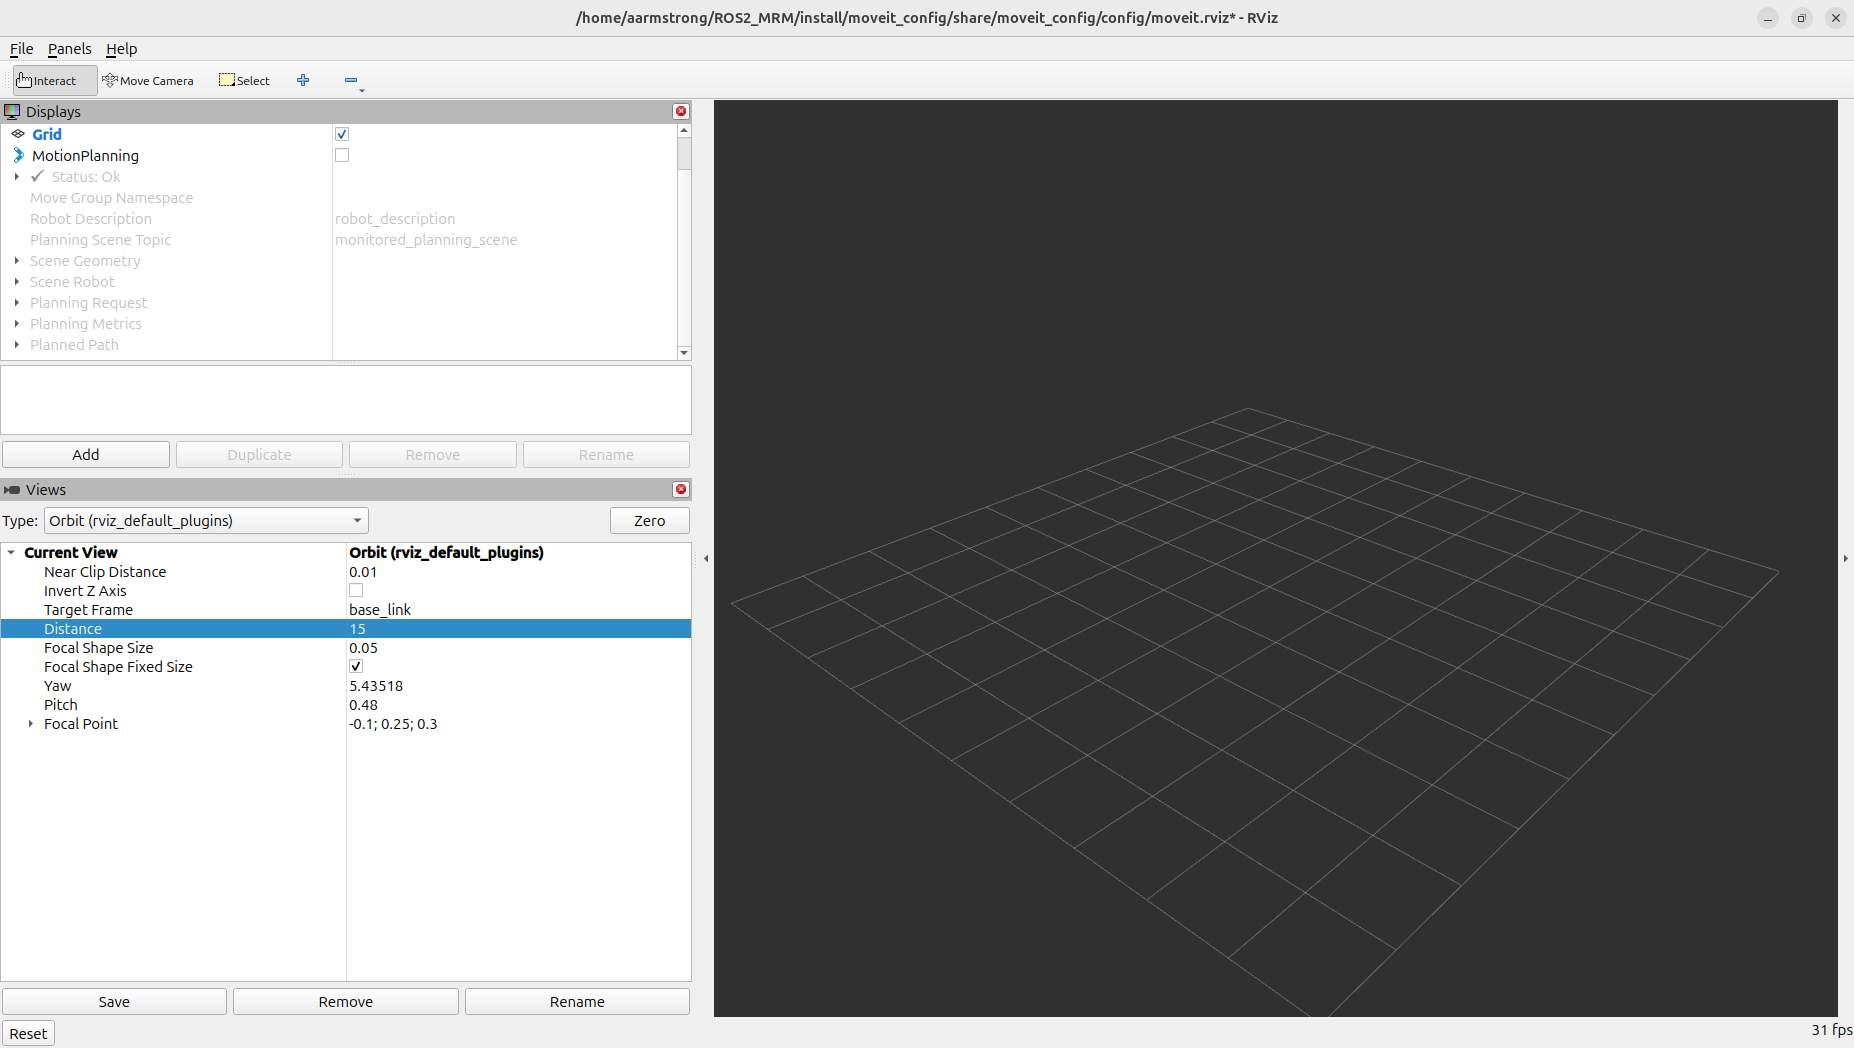
\includegraphics[width=1.0\textwidth]{RViz_Empty.png}
    \caption{RViz2 Empty Grid}
    \label{fig:rviz2_empty_grid}
\end{figure}

To add the URDF model into RViz2, the user can either use the \texttt{robot\_state\_publisher} node to publish the robot's state or manually load the URDF file into RViz2. The \texttt{robot\_state\_publisher} node is a standard ROS2 node that publishes the robot's state based on the URDF model, allowing RViz2 to visualize the robot's kinematic model in real-time. The manual loading of the URDF file can be done by selecting the "Add" button in RViz2 and choosing the "Robot Model" option, then specifying the path to the URDF file by finding the \texttt{Description Topic} in the dropdown menu from the \texttt{RobotModel} Display and subscribing to the \texttt{/robot\_description} topic as can be seen in Figure \ref{fig:rviz2_full_model}. \par

\begin{figure}[ht]
    \centering
    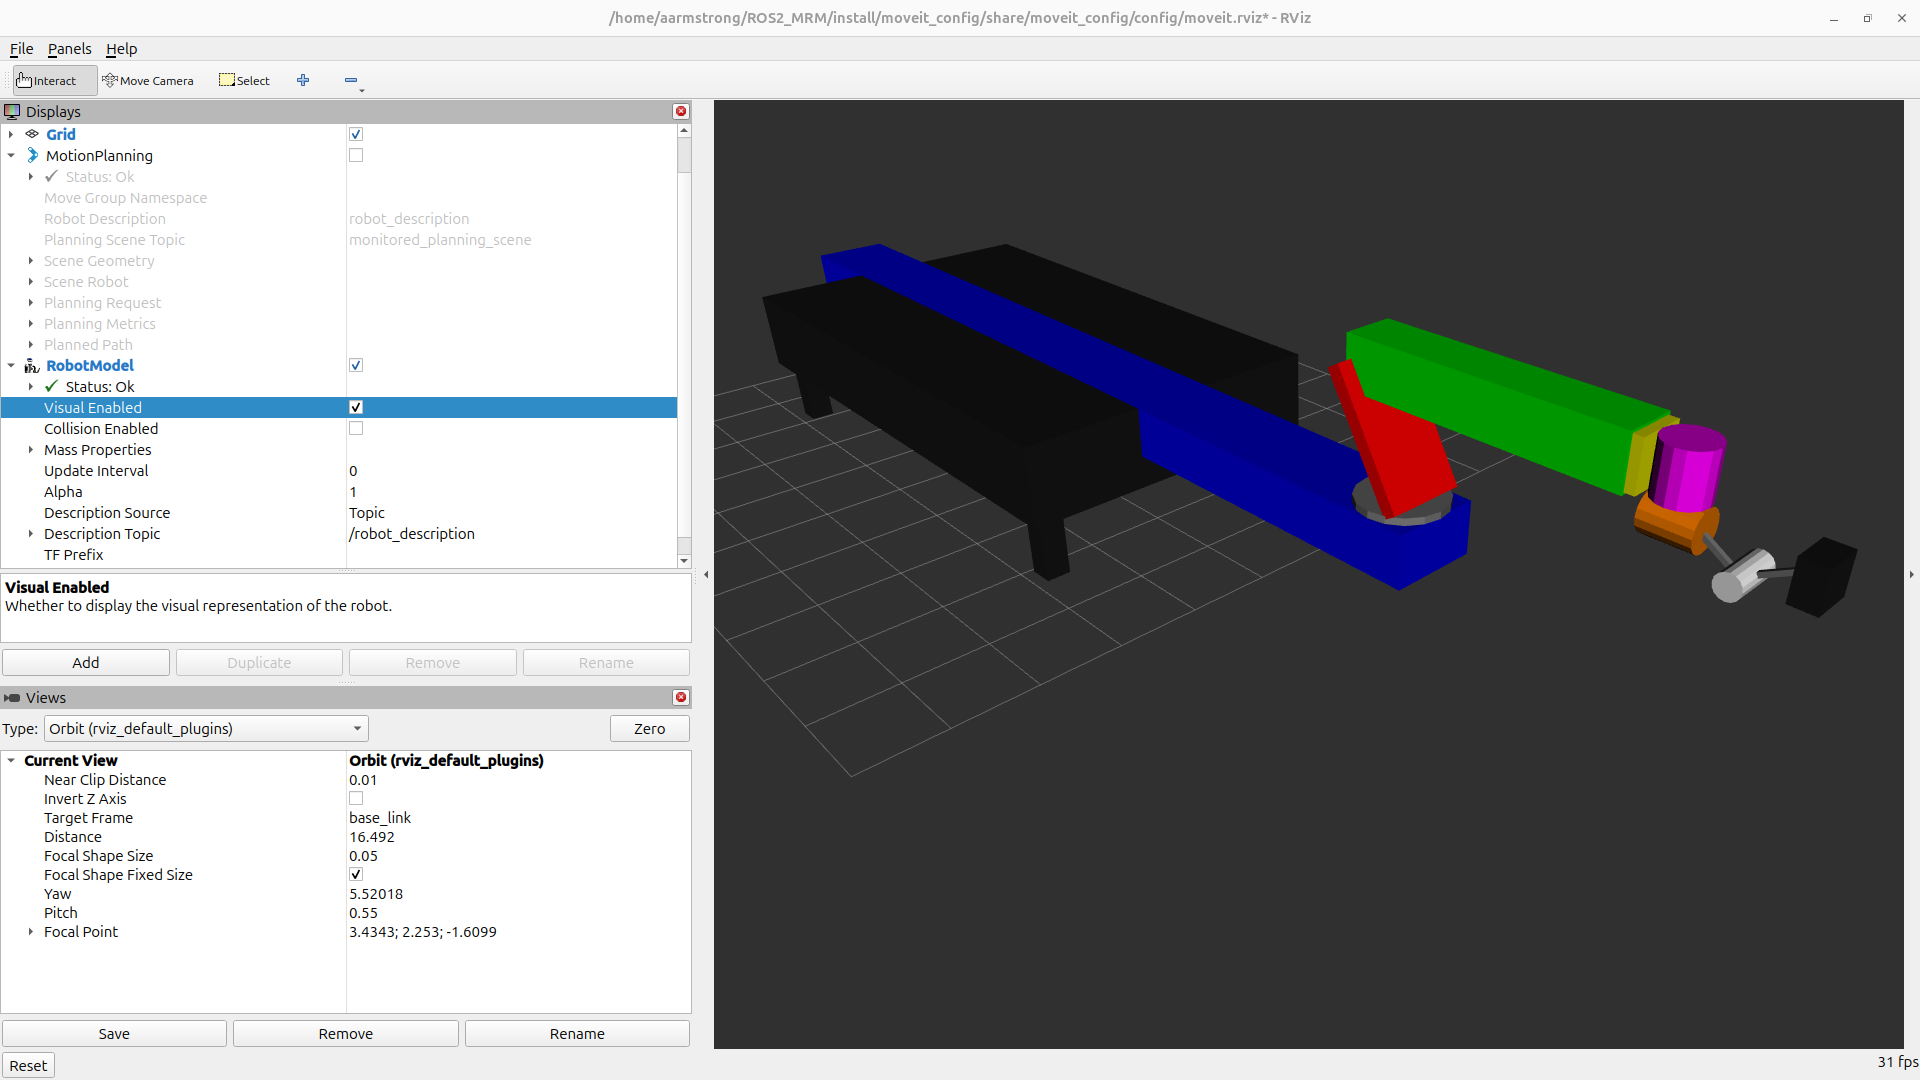
\includegraphics[width=1.0\textwidth]{Full_Model.png}
    \caption{RViz2 Full Model}
    \label{fig:rviz2_full_model}
\end{figure}
\newpage

\begin{wrapfigure}{l}{0.31\textwidth}
    \centering
    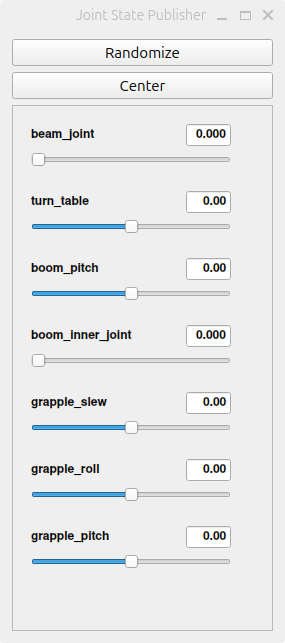
\includegraphics[width=0.3\textwidth]{Joint_State_Publisher.png}
    \caption{RViz2 Joint State Publisher}
    \label{fig:rviz2_joint_state_publisher}
\end{wrapfigure}

Now that the model is loaded and the joints/links have been defined and published, they can be modified at will as the robot's configuration changes - the parameters can be adjusted in the URDF file or through the ROS2 parameter server. The implementation used here was a joint state publisher node that allows the user to manually adjust the joint angles and positions in RViz2, providing a real-time visualisation of the robot's kinematic model. This is particularly useful for testing and debugging the kinematic model before implementing motion planning algorithms and is the recommended method for visualising the robot's model in RViz2 as described by ROS2 documentation. Figure \ref{fig:rviz2_joint_state_publisher} shows the python window used to control the joint states, noting that these values are in radians and are defined by the limits in the URDF file.
\clearpage

Another useful feature of RViz2 is the TF (Transform) visualisation, which displays the coordinate frames of the robot's links and joints. This provides a graphical representation of the robot's kinematic relationships, allowing users to see how the robot's links are connected and how they move relative to each other. The TF visualisation can be enabled by selecting the "TF" option in the RViz2 display panel the same as performed previously when adding the \texttt{Robot Model}, as shown in Figure \ref{fig:rviz2_tf_visualisation}.

\begin{figure}[ht]
    \centering
    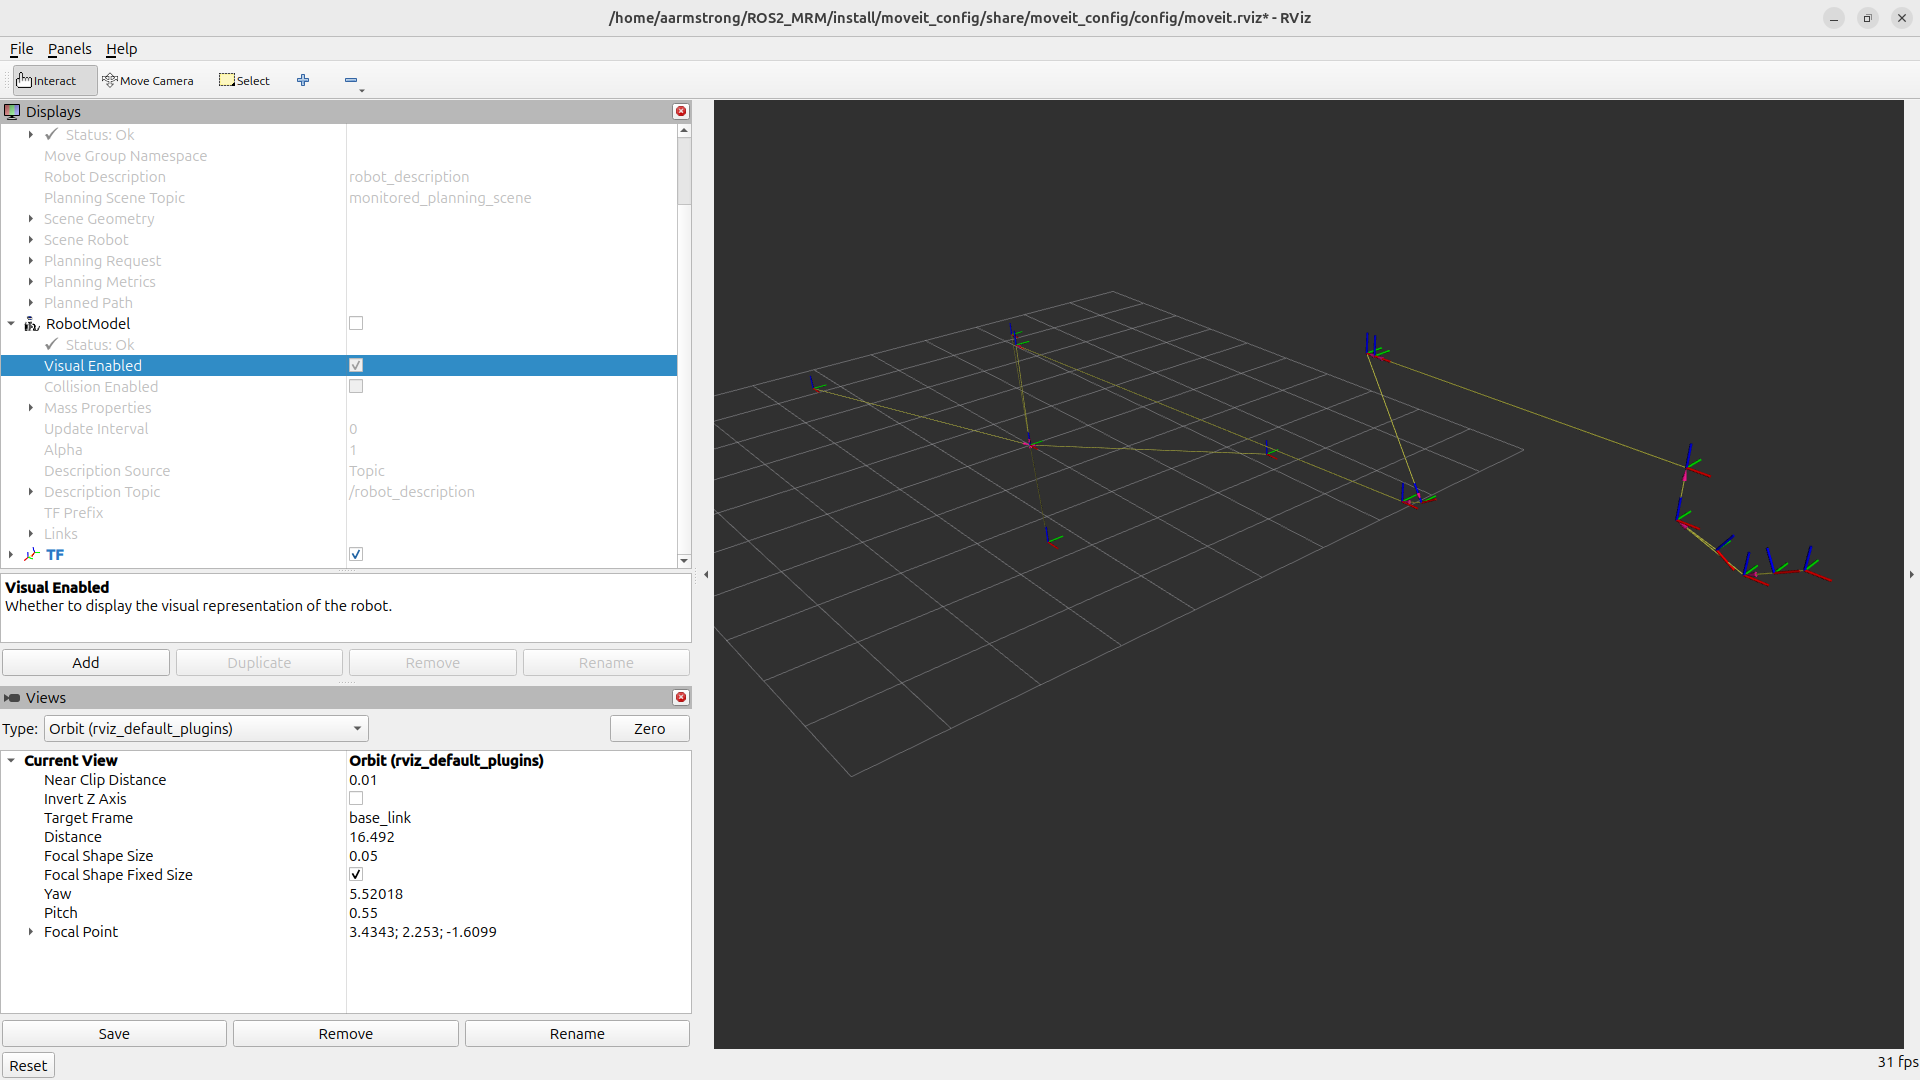
\includegraphics[width=1.0\textwidth]{TF_Visualisation.png}
    \caption{RViz2 TF Visualisation}
    \label{fig:rviz2_tf_visualisation}
\end{figure}

The TF visualisation is quite helpful when constructing the kinematic model from scratch as it show the joint coordinate frames whereas the Robot Model visualisation only shows the boxes/cylinders, remembering that the origin of the joint and the origin of the boxes/cylinders may not be the same. It also gives a visualisation to the links between each joint with arrows and labels indicating the joint coordinate frames. This visualisation is essential for understanding the robot's kinematic relationships and ensuring that the URDF model is correctly defined. It also provides a useful reference for debugging and testing the kinematic model before implementing motion planning algorithms.
\newpage


\subsection{MoveIt2 - Kinematics and Motion Planning Framework}
MoveIt2 is a seperate package used in this investigation to allow for motion planning and kinematic analysis of the robot's model. The motion planning is implemented into RViz2 
The \texttt{MoveIt2} package also provides a number of pre-built motion planning algorithms, including the \texttt{RRTConnect} algorithm, which is a fast and efficient motion planning algorithm.


The \texttt{MoveIt2} package provides capabilities for inverse kinematics calculations through the use of community developed plugins and libraries. You could develop your own plugin to implement a custom inverse kinematics algorithm, but this is not recommended by the MoveIt2 developers unless you have a specific need for a custom algorithm. The \texttt{MoveIt2} package provides a number of pre-built plugins that can be used for inverse kinematics calculations, including the \texttt{KDL} plugin, which is an implementation using the jacobian method of approximation.
The \texttt{KDL} plugin can be called through the \texttt{ros2 service call} command, specifying the appropriate service and message types. The appropriate service in this case is the \texttt{/compute\_ik} service, which is a standard service provided by the \texttt{MoveIt2} package for inverse kinematics calculations and is likely the same service across plugins other than \texttt{KDL}. The message type for this service is \texttt{moveit\_msgs/srv/GetPositionIK}, which must provide the \texttt{group\_name} and the \texttt{pose\_stamped} fields. The \texttt{group\_name} field specifies the name of the robot's kinematic group, which is defined in the URDF file, and the \texttt{pose\_stamped} field specifies the desired pose of the end effector in the robot's coordinate frame, this is passed as a location in \texttt{<x, y, z>} space and \texttt{<x, y, z, w>} orientation. The \texttt{timeout} field specifies the maximum time allowed for the inverse kinematics calculation to complete, and the \texttt{avoid\_collisions} field specifies whether to avoid collisions with other links in the robot's kinematic model, noting that collisions are technically ignored if they are not defined in the URDF anyway. \par

The orientation of the end effector is specified in quaternion notation, which is a mathematical representation of rotation in 3D space. The quaternion is defined by four components: \texttt{x}, \texttt{y}, \texttt{z}, and \texttt{w}, where \texttt{w} is the scalar part and \texttt{x}, \texttt{y}, and \texttt{z} are the vector part. The quaternion can be converted to Euler angles or other representations if needed, but for the inverse kinematics calculations, it is typically used in its quaternion form. \par

Figure \ref{fig:rviz2_ik_calculations} shows the a command input for the inverse kinematics calculations (the cyan box), where the user has specified the desired pose of the end effector and the robot's kinematic group. The position and orientation are clearly defined as floating point numbers even when they are 0 values but this is not mandatory and the command will work if supplied integers. The red box shows our service call being broadcast to the \texttt{/compute\_ik} service and its current values, which are all 0s as per the initial conditions. Finally, the green box in Figure \ref{fig:rviz2_ik_calculations} shows the response from the service which states the joint names and their new positions.

\begin{figure}[ht]
    \centering
    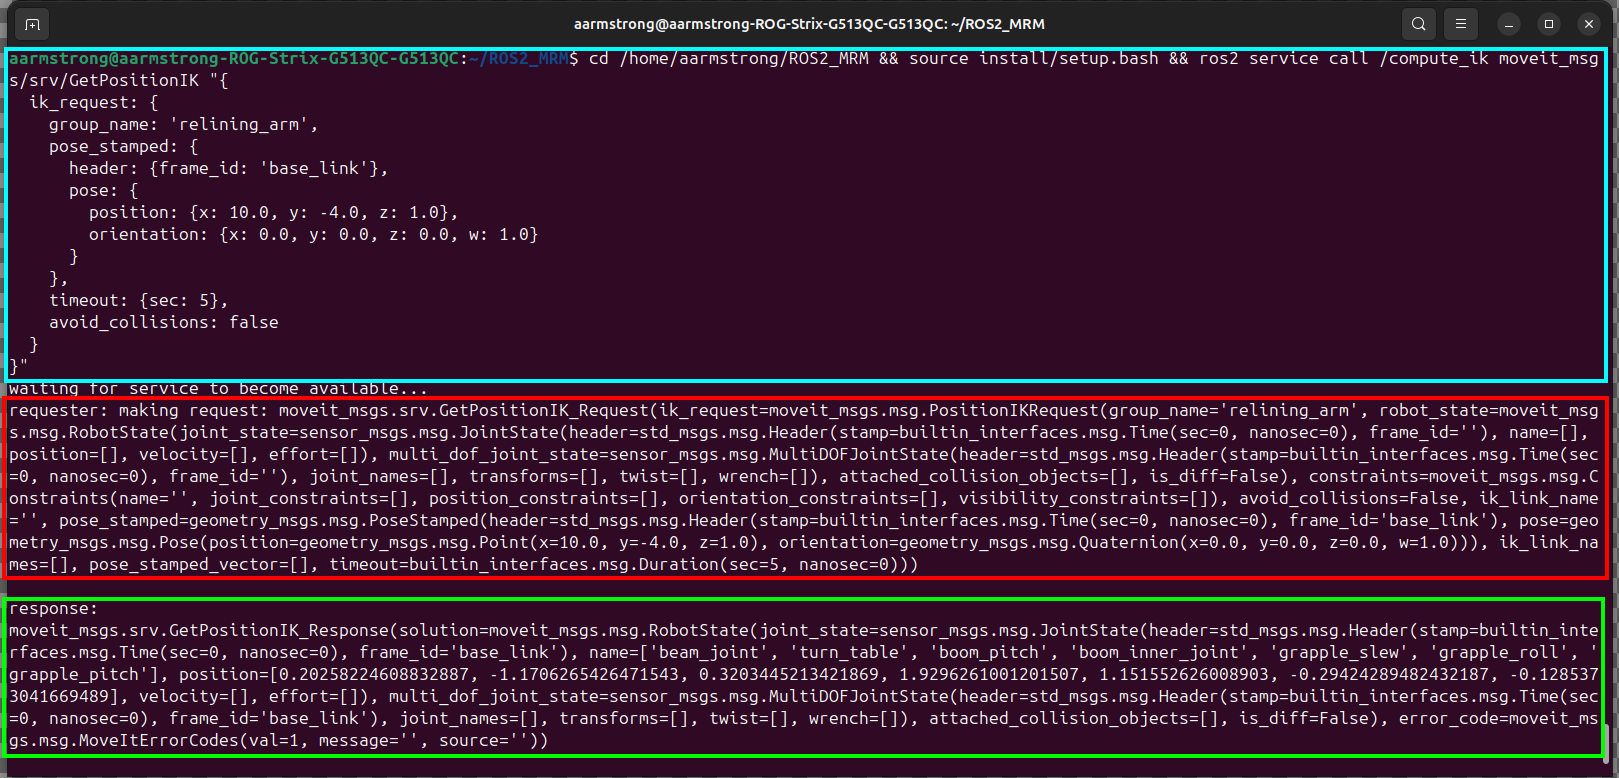
\includegraphics[width=1.0\textwidth]{IK_Calcs_Coloured.png}
    \caption{RViz2 IK Calculations}
    \label{fig:rviz2_ik_calculations}
\end{figure} \newpage

Now that the joint positions have been calculated, they can be published to the \texttt{/joint\_states} topic using the \texttt{ros2 topic pub} command. The message type for this topic is \texttt{sensor\_msgs/msg/JointState}, which contains the joint names and their corresponding positions as they were defined during launch. Figure \ref{fig:rviz2_ik_publisher} shows the command used to publish the joint states to the \texttt{/joint\_states} topic, where the joint names and their corresponding positions are all specified at once. Specifying all joints and their changes at once is not necessary and a user may only wish to change a single joint's position at a time to view only that joint's movement. The positions are specified as floating point numbers, which can entered as integers, and are defined in radians for rotational joints and meters for prismatic joints. The command will publish the joint states to the topic, allowing other nodes to subscribe to the topic and receive the updated joint positions. It should also be noted that the \texttt{ros2 topic pub} command will publish the joint states repeatedly at the ROS operating frequency, which is typically 10Hz, until the command is stopped. The \texttt{--once} flag can be used to publish the joint states only once, which is useful for testing and debugging purposes. As before the first block of text shows the published command and the second block shows the response from the service.

\begin{figure}[ht]
    \centering
    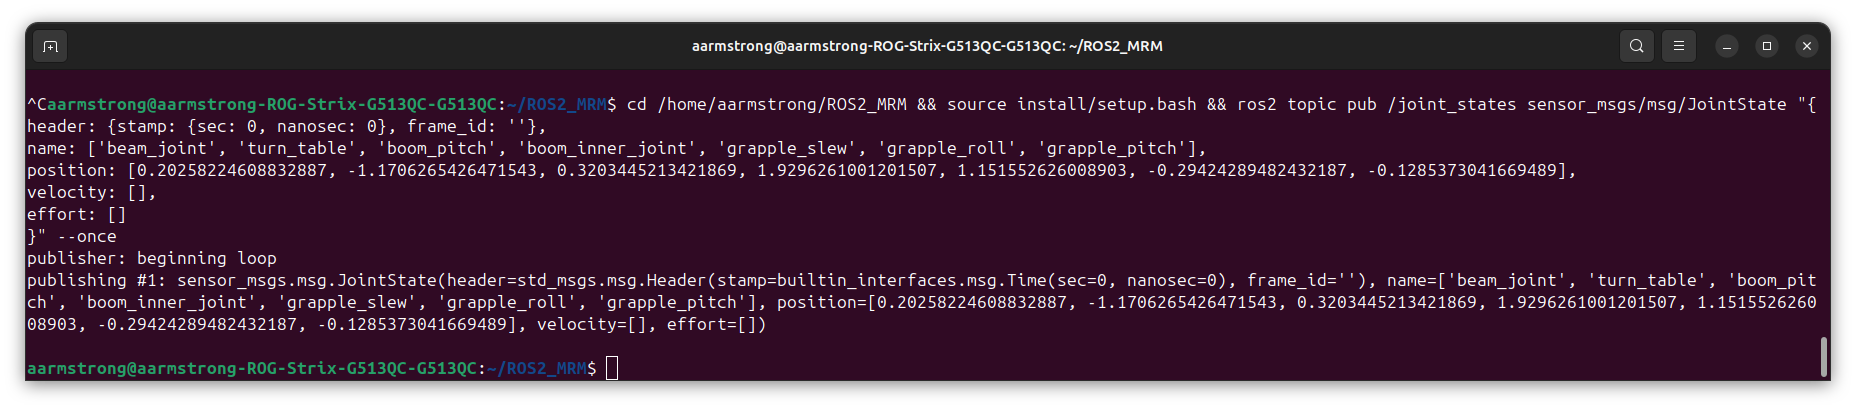
\includegraphics[width=1.0\textwidth]{IK_Publisher.png}
    \caption{RViz2 IK Publisher}
    \label{fig:rviz2_ik_publisher}
\end{figure}

After the joint values have been published they can be visualized in RViz2. The motion planning tab should already be displaying the robot model and the user should now see that the robot has moved into its new position. Figure \ref{fig:rviz2_ik_rviz_publisher} shows the RViz2 interface containing the robot arm's original position and orientation (in orange) and its new position and orientation.

\begin{figure}[ht]
    \centering
    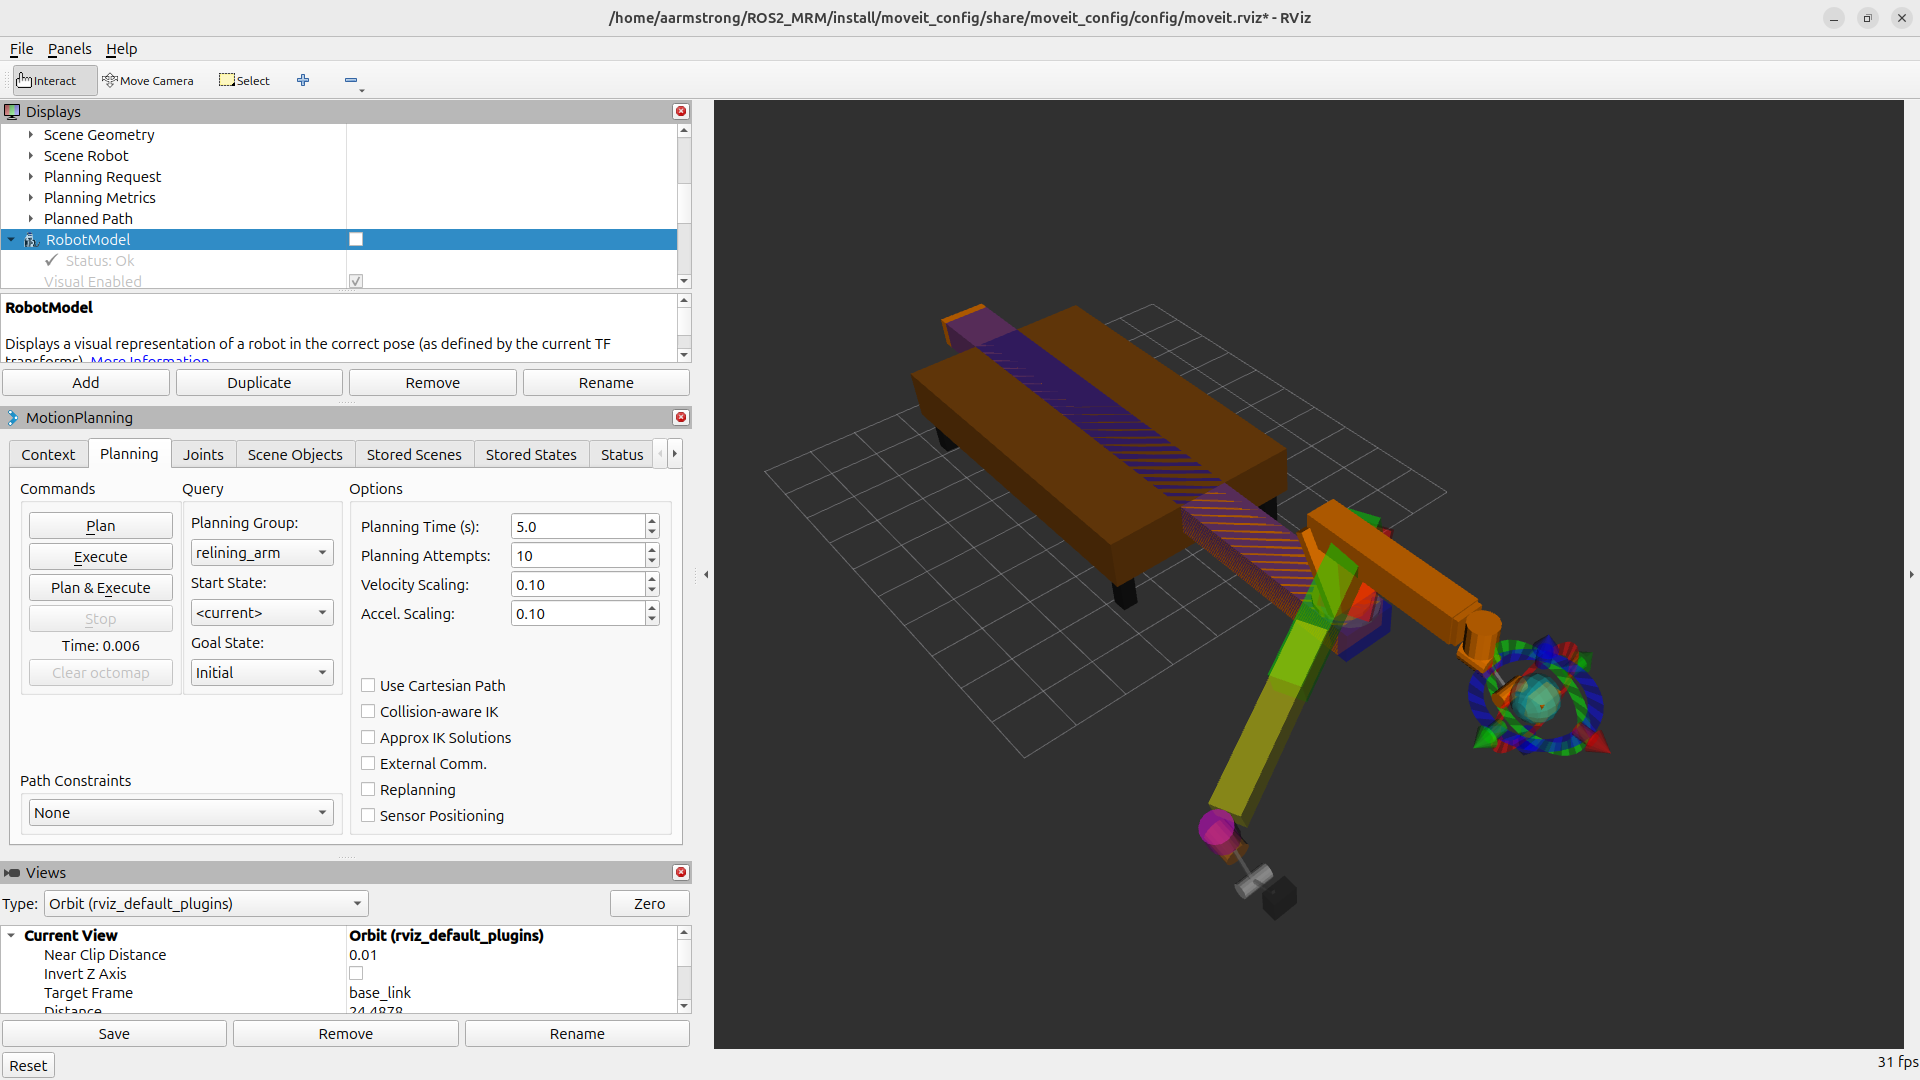
\includegraphics[width=1.0\textwidth]{IK_RViz_Publisher.png}
    \caption{RViz2 IK Publisher}
    \label{fig:rviz2_ik_rviz_publisher}
\end{figure}
\newpage

\begin{comment}
cd /home/aarmstrong/ROS2_MRM && source install/setup.bash && ros2 service call /compute_ik moveit_msgs/srv/GetPositionIK "{
  ik_request: {
    group_name: 'relining_arm',
    pose_stamped: {
      header: {frame_id: 'base_link'},
      pose: {
        position: {x: 10.0, y: -4.0, z: 1.0},
        orientation: {x: 0.0, y: 0.0, z: 0.0, w: 1.0}
      }
    },
    timeout: {sec: 5},
    avoid_collisions: {false}
  }
}"

cd /home/aarmstrong/ROS2_MRM && source install/setup.bash && ros2 topic pub /joint_states sensor_msgs/msg/JointState "{
header: {stamp: {sec: 0, nanosec: 0}, frame_id: ''},
name: ['beam_joint', 'turn_table', 'boom_pitch', 'boom_inner_joint', 'grapple_slew', 'grapple_roll', 'grapple_pitch'],
position: [1.4266798804799865, 0.9345235988712364, 0.6436777249998131, 1.5327355954379027, 1.2125009942113316, -0.6124892088326688, -1.1393371486253658],
velocity: [],
effort: []
}" --once


PODMAN  docker services
\end{comment}



\section{Future Research - Not implemented in this study}
This section includes areas that were researched but not implemented in this investigation. These areas are left for future research and development to further enhance the capabilities of the mill relining robot and potentially improve the utility of ROS2 in RME practices.

\begin{itemize}
    \item Implementation of sensors and sensor-based algorithms for improved perception.
    \item Implementation of collision based path-planning with foreign objects (mill liners, equipment, etc.)
    \item Exploration of multi-robot collaboration for complex tasks including liner-cart operations.
\end{itemize}

\subsection{Sensors}
The ROS2 libraries that allow for control over the robot model via sensors are called the \texttt{ROS2 Control} libraries. These libraries provide a framework for integrating sensors and actuators into the ROS2 ecosystem, allowing for "real-time" data acquisition and control of the robot's hardware components. The documentation for the corresponding version of the \texttt{ROS2 Control} libraries can be found on the official \href{https://control.ros.org/kilted/doc/getting_started/getting_started.html#}{ROS2 website} and details the architecture and implementation but does assume a rather high baseline understanding of ROS concepts.

The architecture is as follows:
\begin{itemize}
  \item The \textbf{Controller Manager} is responsible for initially loading the controllers and connecting them to their hardware abstracted sides of the ROS2\_control framework. This is also the user's entry point. The controller manager is a node that does have indirect access (through the resource manager) to the hardware components and their interfaces to allow or matching the required and provided interfaces.
  \item The \textbf{Resource Manager} is responsible for the physical hardware abstraction and its drivers. It loads their states and their command interfaces. The abstraction is ideal for reuse of implemented hardware components without any additional implementations and flexible hardware application for state and command interfaces, separate hardware/communication libraries for motor control and encoder reading.
  \item The \textbf{Controllers} compare the reference value with the measured output and, based on that error, calculate the system's input.
  \item The \textbf{User Interfaces} are an easier implementation of service calls directly from the command line by providing a number of auto-complete and predefined command functions to aid the user's use of direct command line inputs.
\end{itemize}

\noindent There is also a number of basic hardware components:
\begin{itemize}
  \item \textbf{System}: Complex (multi-DOF) robotic hardware like industrial robots. The main difference between the Actuator component is the possibility to use complex transmissions like needed for humanoid robot's hands. This component has reading and writing capabilities. It is used when there is only one logical communication channel to the hardware.
  \item \textbf{Actuators}: Simple (1 DOF) robotic hardware like motors, valves, and similar. An actuator implementation is related to only one joint. This component type has reading and writing capabilities. Reading is not mandatory if not possible (e.g., DC motor control with Arduino board). The actuator type can also be used with a multi-DOF robot if its hardware enables modular design, e.g., CAN-communication with each motor independently.
  \item \textbf{Sensors}: Robotic hardware is used for sensing its environment. A sensor component is related to a joint (e.g., encoder) or a link (e.g., force-torque sensor). This component type has only reading capabilities.
\end{itemize}
Further reading about hardware can be found in this \href{https://github.com/ros-controls/roadmap/blob/master/design_drafts/hardware_access.md}{github documentation}

The ROS2\_control framework uses the <ros2\_control>-tag in the robot's URDF file to describe its components, i.e., the hardware setup. The chosen structure enables tracking together multiple xacro-macros into one without any changes. The example hereunder, Figure \ref{fig:ros2_control_urdf}, shows a position-controlled robot with 2-DOF (RRBot), an external 1-DOF force-torque sensor, and an externally controlled 1-DOF parallel gripper as its end-effector.
\begin{figure}[ht]
    \centering
    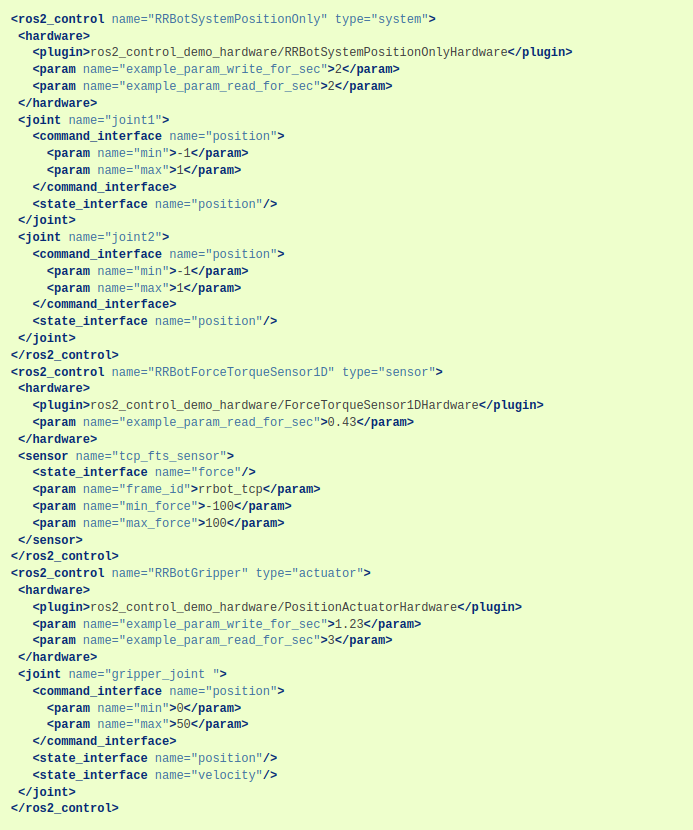
\includegraphics[width=0.8\textwidth]{ROS2_Control_URDF.png}
    \caption{ROS2 Control URDF Example}
    \label{fig:ros2_control_urdf}
\end{figure} \clearpage
To make use of this the usual configuration YAML file of the controller manager, the rest of the URDF file contents with robot joints and visualisation, and the launch files with the nodes and their configurations must also be created/included.

\subsection{Obstacle Collision Based Path Planning}
\texttt{MoveIt2} does have collision capabilities and are used in a minor extent for checking the joints haven't collided with each other in order to reach a point, but obstacle collision based path planning capabilities are not implemented in this investigation. Obstacle collision based path planning is implemented through the use of sensors and sensor-based algorithms, which allow the robot to detect and avoid obstacles in its environment and plan around them. Additionally, better collision based path planning can implemented through higher-speed sensor calculations make by a package named \texttt{Nav2 Collision Monitor}. Its documentation can be found \href{https://index.ros.org/p/nav2_collision_monitor/#kilted}{here}. The basics is that the \texttt{Nav2 Collision Monitor} package provides a framework for faster collision avoidance where an obstacle "appears out of nowhere" from the robot's perspective, allowing for more responsive and adaptive path planning.

\subsection{Multi-Robot Collaboration}
Multi-robot collaboration is a complex topic that involves coordinating multiple robots to work together on a task. This can include tasks such as transporting objects, performing complex operations, or working together to achieve a common goal. The ROS2 framework does not have a native multi-robot collaboration package, but does of course have community support built upon the ROS2 framework. This additional framework is called the \texttt{Robotics Middleware Framework} 
RMF is a set of tools and specifications designed for integrating and managing multi-robot systems. Key points include:
\begin{itemize}
  \item \textbf{RMF Core:} It includes components like rmf\_traffic for traffic management, rmf\_task for task planning, and rmf\_battery for battery estimation.
  \item \textbf{Traffic Deconfliction:} RMF provides traffic conflict prevention and resolution through a centralized Traffic Schedule Database. It also employs a negotiation scheme to resolve conflicts.
  \item \textbf{Fleet Adapters:} These connect fleet-specific APIs to RMF, handling communication with smart infrastructure. Four levels of control are provided, from full control to traffic light control, each offering different capabilities for managing robot fleets.
\end{itemize}

This framework aims to facilitate the integration and interoperability of robotic systems, creating coordination and messaging across multiple robots and fleets. It is particularly useful in environments where multiple robots need to work together. The framework is designed to be modular and extensible, allowing for easy integration with existing robotic systems and the addition of new capabilities as needed. The RMF framework is still under development and is not yet fully integrated into the ROS2 ecosystem.
Further reading about the RMF can be found \href{https://osrf.github.io/ros2multirobotbook/intro.html}{here}.
\newpage



\section{Conclusion}
This investigation has explored the use of ROS2 and its associated packages for the development of a mill relining robot. The kinematic model was constructed using URDF and Xacro files, allowing for a modular and scalable representation of the robot's physical structure. The MoveIt2 package was used to implement motion planning algorithms, enabling real-time trajectory generation and optimization. The RViz2 visualization tool provided a graphical interface for visualizing the robot's state, motion planning, and planned trajectories.
The investigation has demonstrated the capabilities of ROS2 for developing complex robotic systems, including the integration of sensors, motion planning, and visualization. The use of ROS2 and its associated packages has enabled the development of a flexible and extensible framework for the mill relining robot, allowing for easy integration of new capabilities and the addition of new sensors and actuators as needed. The investigation has also highlighted the importance of modularity and scalability in the design of robotic systems, allowing for easy updates and modifications to the kinematic model without affecting the entire system. The use of Xacro files has significantly reduced redundancy in the URDF files, making them easier to maintain and extend whilst increasing readability. The investigation has also demonstrated the importance of visualization tools such as RViz2 for debugging and testing the kinematic model, providing a real-time visual representation of the robot's state and motion planning. The use of MoveIt2 has enabled the implementation of motion planning algorithms, allowing for real-time trajectory generation and optimization.



\end{document}